\subsection{ResNet50}\label{resnet50}
\chapterauthor{Benjamin Loh Choon How (2201590)}

The ResNet50 model is a convolutional neural network (CNN) architecture that represents a significant evolution in deep learning technologies. Developed by Microsoft Research, it introduced the novel concept of residual learning to address the challenges of training very deep neural networks. ResNet50 is particularly notable for its use of "skip connections," which help to prevent the vanishing gradient problem by allowing gradients to flow through an alternative shortcut path across layers.

At its core, ResNet50 builds upon the successes of earlier CNNs but with deeper architectures made feasible through these residual connections. This allows the network to learn from a significantly increased number of layers without a corresponding degradation in performance, leading to more accurate and efficient models. Widely adopted in various applications, ResNet50 excels in tasks such as image classification, object detection, and increasingly in areas requiring fine-grained visual understanding. The model's design is an improved iteration over its predecessors, making it a cornerstone in the field of deep learning for handling complex visual tasks with remarkable effectiveness.

\subsubsection{Implementation}

The proposed brain tumor classification model is built upon the ResNet50 architecture, pretrained on the ImageNet dataset. The top layers of the ResNet50 model are excluded to customize it for our specific classification task. The input shape is set to $224\times224$ with three channels, accommodating the resizing of input images during preprocessing to match these dimensions. This modification is essential to align the image dimensions with the network's input requirements, thereby enhancing the classification accuracy.

To adapt the model for brain tumor classification, the output of the ResNet50 base model undergoes a Global Average Pooling operation. This layer effectively reduces the spatial dimensions of the feature maps to a single value per map, preserving essential features while minimizing the model complexity. A Dropout layer with a rate of 0.4 is added subsequently to mitigate overfitting by randomly dropping a fraction of neurons during training, ensuring robust generalization. The final classification layer is a Dense layer with four neurons, each representing one of the brain tumor classes: meningioma, glioma, pituitary, and notumor. A softmax activation function is employed in this layer to output class probabilities, providing a clear probabilistic interpretation of the predictions.

The model is compiled with the Adam optimizer, set to a learning rate of $0.0001$, and the categorical cross-entropy loss function. This choice of optimizer and loss function is ideal for our multi-class classification task, offering a balance between rapid convergence and precise adjustments during training. The model's performance metrics include accuracy, ensuring a comprehensive evaluation of its effectiveness.

Training is conducted with a series of callbacks to optimize performance and prevent overfitting. These include ModelCheckpoint to save the model with the lowest validation loss and EarlyStopping to halt training when no improvement in validation loss is observed for a specified number of epochs. Training was performed over 80 epochs but early stopped at epoch 50, with a batch size of 10, and was trained on the training set and validated on the validation set. The model with the best validation accuracy was saved as the final model. The model was then evaluated on the test set to obtain the final performance metrics. The model achieved an accuracy of 0.9973 and a validation accuracy of 0.9111, with a validation loss of 0.2656. The model's performance metrics are summarized in Table \ref{tab:resnet50_classification_report} and Table \ref{tab:resnet50_additional_metrics}.

\subsubsection{Fine-Tuning}

In the fine-tuning phase of the ResNet50 model, the Optuna package was employed to systematically explore and optimize the hyperparameters, particularly focusing on the dropout rate. The goal of this process was to identify the most effective dropout rate that balances model performance and overfitting. Through multiple trials, each testing a different dropout rate within the range of 0.1 to 0.5, the optimal dropout rate was found to be 0.4, which provided a balance between mitigating overfitting and maintaining model performance. This specific dropout rate was thus adopted in the final model architecture.

The overall approach demonstrates the rigorous method employed to fine-tune the model, ensuring optimal performance for brain tumor segmentation. By leveraging advanced optimization techniques and thoroughly validating the model, this work contributes to the development of more accurate and reliable medical imaging models.

\subsubsection{Results and Evaluation}

\begin{figure}[H]
  \centering
  \begin{subfigure}[b]{0.2\textwidth}
    \centering
    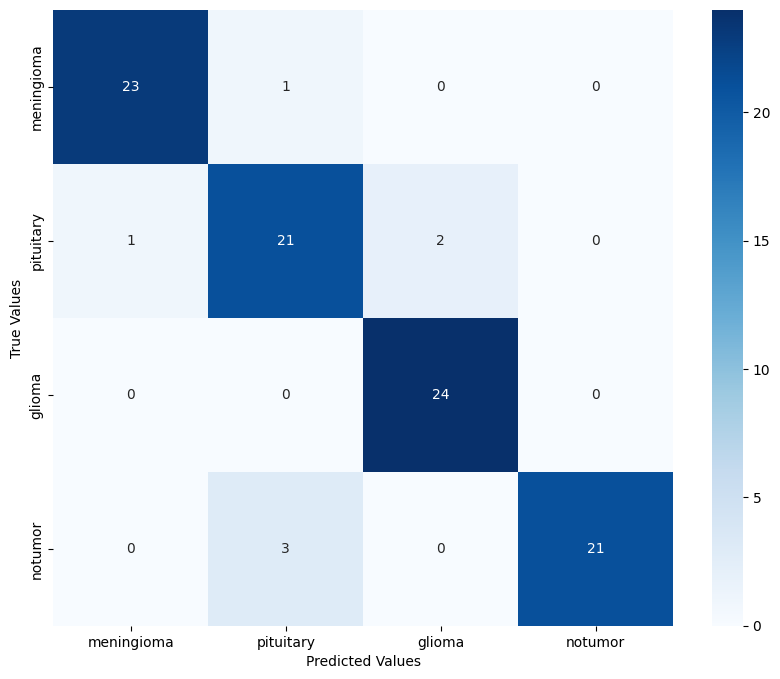
\includegraphics[width=\textwidth]{resnet50/evaluation/cm1.png}
    \caption{Confusion Matrix}
    \label{fig:resnet50_cm1}
  \end{subfigure}
  \hfill
  \begin{subfigure}[b]{0.2\textwidth}
    \centering
    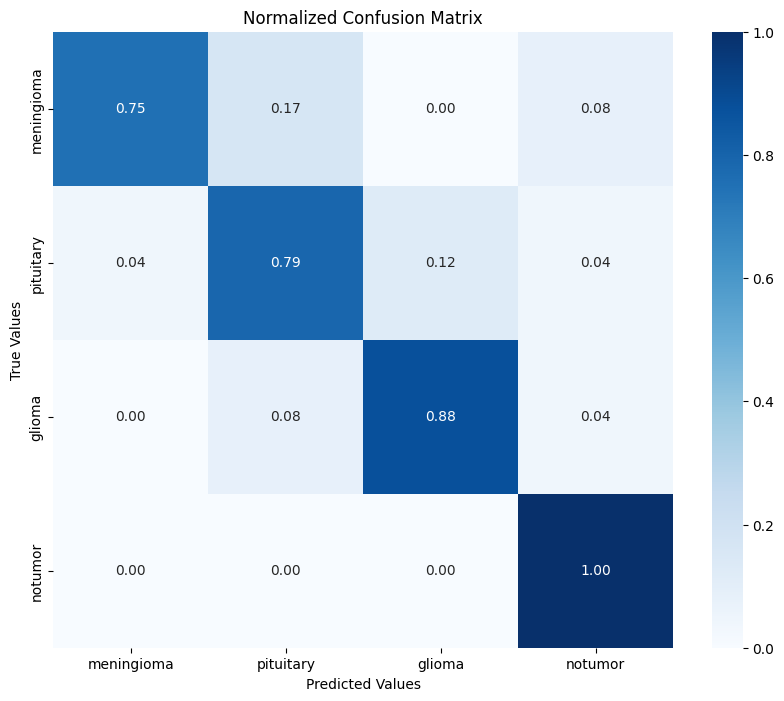
\includegraphics[width=\textwidth]{resnet50/evaluation/cm2.png}
    \caption{Normalized Confusion Matrix}
    \label{fig:resnet50_cm2}
  \end{subfigure}
  \hfill
  \begin{subfigure}[b]{0.25\textwidth}
    \centering
    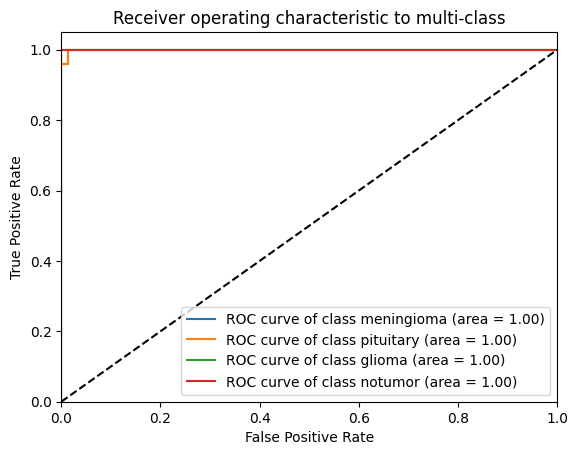
\includegraphics[width=\textwidth]{resnet50/evaluation/ROC.png}
    \caption{ROC Curve}
    \label{fig:resnet50_roc}
  \end{subfigure}
  \hfill
  \begin{subfigure}[b]{0.25\textwidth}
    \centering
    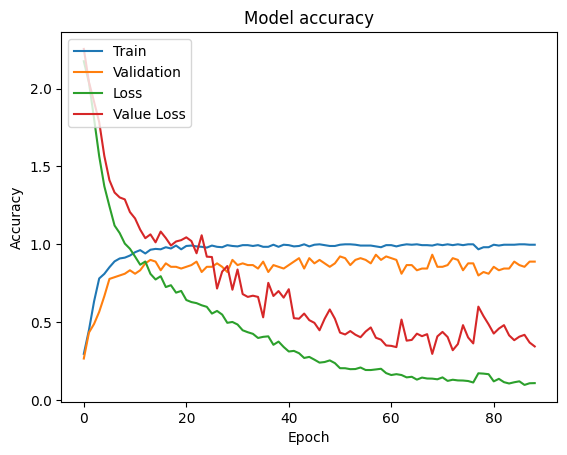
\includegraphics[width=\textwidth]{resnet50/evaluation/learning_curve.png}
    \caption{Learning Curve}
    \label{fig:resnet50_learning_curve}
  \end{subfigure}
  \caption{Confusion Matrix, Normalized Confusion Matrix, ROC Curve, and Learning Curve for Brain Tumor Segmentation}
  \label{fig:resnet50_evaluation}
\end{figure}

\begin{longtable}{|l|c|c|c|c|}
\caption{Classification Report for Brain Tumor Segmentation} \label{tab:resnet50_classification_report}
\hline \textbf{Class} & \textbf{Precision} & \textbf{Recall} & \textbf{F1-Score} & \textbf{Support}
\hline 
\endfirsthead

\multicolumn{5}{c}%
{{\bfseries \tablename\ \thetable{} -- continued from previous page}}
\hline \textbf{Class} & \textbf{Precision} & \textbf{Recall} & \textbf{F1-Score} & \textbf{Support} 
\hline 
\endhead

\hline \multicolumn{5}{|r|}{{Continued on next page}} 
\hline
\endfoot

\hline
\endlastfoot

glioma      & 0.88 & 0.88 & 0.88 & 24 \\ 
\hline
meningioma  & 0.83 & 0.79 & 0.81 & 24 \\ 
\hline
notumor     & 0.89 & 1.00 & 0.94 & 24 \\ 
\hline
pituitary   & 1.00 & 0.92 & 0.96 & 24 \\ 
\hline
micro avg   & 0.90 & 0.90 & 0.90 & 96 \\ 
\hline
macro avg   & 0.90 & 0.90 & 0.90 & 96 \\ 
\hline
weighted avg & 0.90 & 0.90 & 0.90 & 96 \\ 
\hline
samples avg & 0.90 & 0.90 & 0.90 & 96 \\ 
\end{longtable}

\begin{longtable}{|c|c|c|c|}
\caption{Additional Metrics for Brain Tumor Segmentation} \label{tab:resnet50_additional_metrics}
\hline 
\textbf{DSC} & \textbf{Sensitivity} & \textbf{Specificity} & \textbf{Accuracy}
\hline
\endfirsthead

\multicolumn{4}{c}%
{{\bfseries \tablename\ \thetable{} -- continued from previous page}}
\hline \textbf{DSC} & \textbf{Sensitivity} & \textbf{Specificity} & \textbf{Accuracy} \hline
\endhead

\hline \multicolumn{4}{|r|}{{Continued on next page}} 
\hline
\endfoot

\hline
\endlastfoot

0.8953 & 0.8958 & 0.9652 & 0.8958 \\
\end{longtable}

The confusion matrices in Figures \ref{fig:resnet50_cm1} and \ref{fig:resnet50_cm2}, provide a detailed view of the model's performance across the four brain tumor classes: meningioma, pituitary, glioma, and no tumor. The glioma and meningioma classes exhibit slightly lower but still commendable true positive rates of 0.88 & 0.79 respectively, indicating strong performance across all categories. The classification report in Table \ref{tab:resnet50_classification_report} summarizes the precision, recall, and F1-score for each class. The model demonstrates high precision and recall across all classes, with a notable F1-score of 0.96 for the pituitary class. The overall micro, macro, and weighted averages for precision, recall, and F1-score all stand at 0.90, reflecting consistent and reliable performance.

The ROC curve in Figure \ref{fig:resnet50_roc} displays the true positive rate against the false positive rate for each class. The areas under the curve (AUC) for pituitary and no tumor classes are both perfect at 1.00, while meningioma and glioma classes show AUCs of 0.96 and 0.99, respectively, indicating excellent discriminative ability of the model.

The learning curve in Figure \ref{fig:resnet50_learning_curve} illustrates the model's accuracy and loss over 50 epochs. The plot shows the progression of training and validation accuracy, as well as loss and validation loss. The training accuracy remains relatively stable, while the validation accuracy also shows a stable trend, indicating effective learning. The training loss decreases gradually, and the validation loss fluctuates but generally maintains a downward trend. These trends suggest that the model is learning effectively without significant overfitting, as the validation metrics align closely with the training metrics. However, some oscillations in the validation loss curve may indicate areas for further optimization.

Table \ref{tab:resnet50_additional_metrics} highlights the Dice Similarity Coefficient (DSC), sensitivity, specificity, and accuracy of the model. The DSC of 0.8953 indicates a good overlap between the predicted and actual tumor regions, reflecting the model's proficiency in segmentation tasks. The sensitivity and accuracy, both at 0.8958, demonstrate the model's capability to correctly identify true positives with a high degree of precision. Additionally, the specificity of 0.9652 highlights the model's effectiveness in accurately identifying true negatives, ensuring reliable performance in distinguishing between different classes of brain tumors.

\subsubsection{K-Folds Cross-Validation}

\begin{figure}[H]
  \begin{center}
    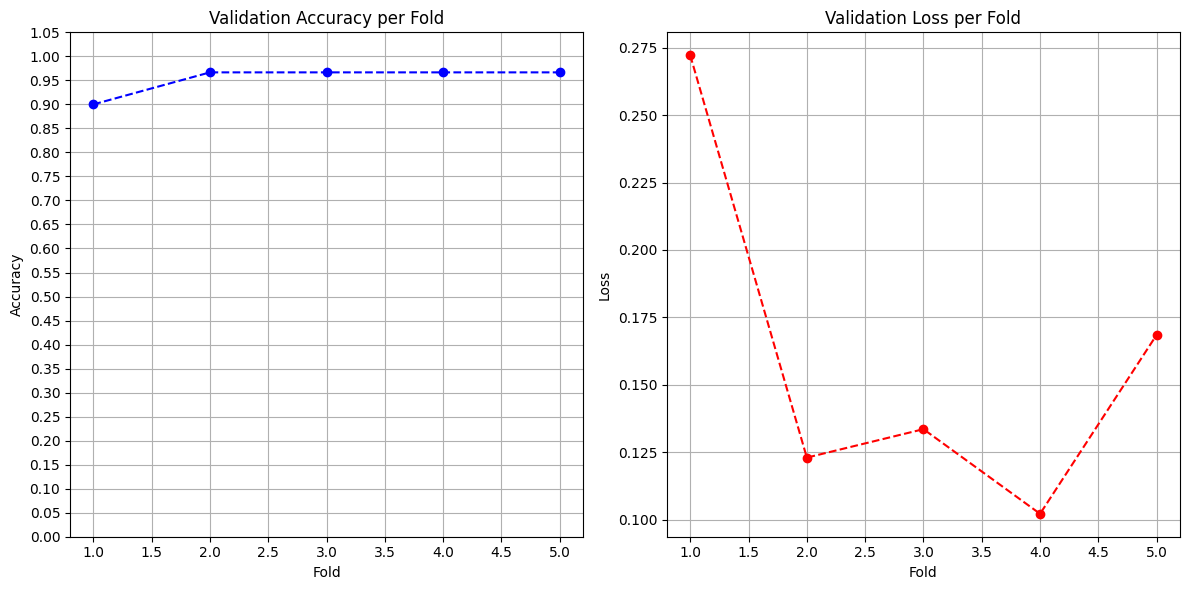
\includegraphics[width=0.7\textwidth]{resnet50/evaluation/kfolds.png}
  \end{center}
  \caption{K-Folds Cross-Validation for Brain Tumor Segmentation}\label{f:resnet50_kfolds}
\end{figure}




% ResNet50, a revolutionary architecture in the field of deep learning, employs residual connections which are its defining feature. These connections are crucial for training very deep networks by enabling the direct propagation of gradients from deeper to shallower layers in the network. This architectural choice reduces the problem of vanishing gradients, thus allowing the model to learn effectively even when many layers deep.

% For our brain tumor classification task, we utilize the ResNet50 model pre-trained on the ImageNet dataset. This pre-training provides a robust feature extraction base, which we then tailor to our specific task through further training and adaptation.

% \textbf{Model Architecture:} Our adaptation of ResNet50 begins with the standard base architecture loaded with ImageNet weights, but excludes the top layer to accommodate our specialized output needs. This modification allows the network to maintain the intricate feature extraction capabilities developed through ImageNet training while adapting to the nuances of brain tumor imagery.

% \begin{quote}
% Imagine ResNet50 like a skilled artisan skilled in restoration. This artisan (the model) is brought into a renovation project (our classification task) where the fundamental structure is sound but needs adaptation and specific enhancements. Just as an artisan would preserve valuable original elements while updating others, our model retains valuable pre-learned features while adapting to new data.
% \end{quote}

% Following the base layers, a Global Average Pooling 2D layer is introduced. This layer reduces the spatial dimensions of the feature maps to a single vector per map, thus summarizing the most critical features while significantly reducing the number of parameters and the computational burden. This pooling step is crucial for maintaining efficiency and avoiding overfitting.

% Next, we include a Dropout layer with a 40\% drop rate, which randomly disables a fraction of the neurons during training. This randomness helps to prevent overfitting by ensuring that the model does not rely too heavily on any specific set of neurons, encouraging the network to develop redundant pathways to maintain performance even if some neurons are inactive.

% The network culminates in a Dense layer with four units corresponding to the different classes of brain tumors, employing the softmax activation function. This layer outputs the probability distribution over the tumor classes, providing a clear, interpretable classification result.

% \textbf{Compilation and Callbacks:} The model is compiled using the Adam optimizer with a starting learning rate of 0.0001 and a loss function of categorical crossentropy, which is appropriate for this multi-class classification scenario. To optimize training, we employ several callbacks:

%     \textit{ModelCheckpoint} to save the best version of the model based on validation loss
%     \textit{EarlyStopping} to halt training if the validation loss does not improve for a specified number of epochs, preventing overtraining and resource wastage

% % to add graph
